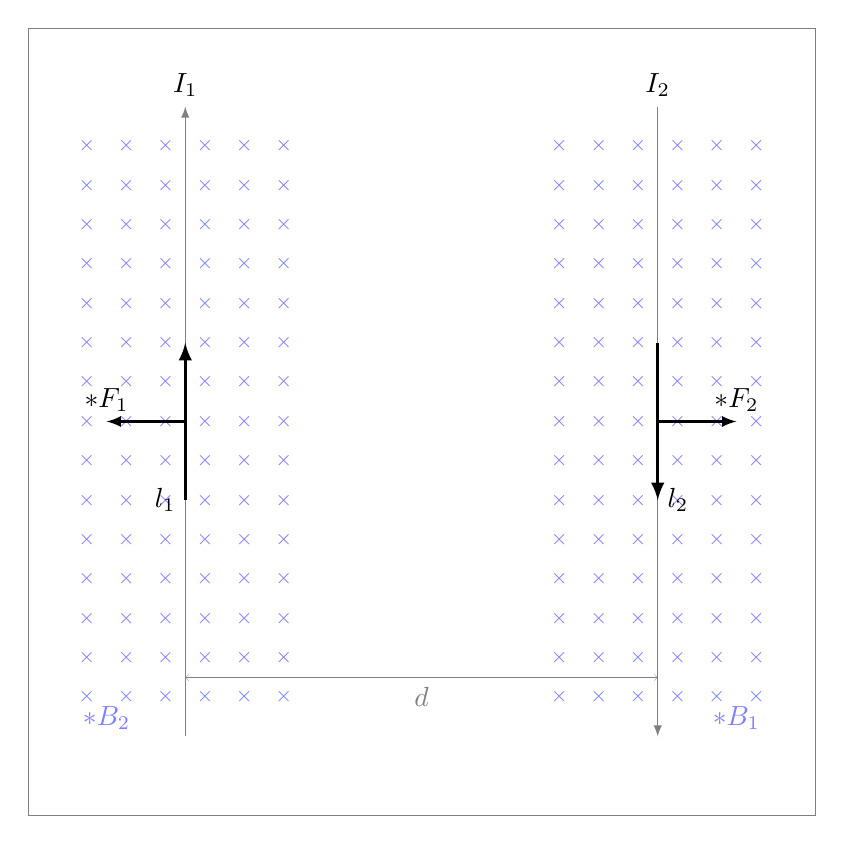
\begin{tikzpicture}[scale=1]
    \draw[gray,ultra thin] (-5,-5) rectangle (5,5);

    \draw[-latex,gray,thin](-3,-4)--(-3,+4) node[above,black] {$I_1$};
    \draw[latex-,gray,thin](+3,-4)--(+3,+4) node[above,black] {$I_2$};

    \foreach \x in {-4.25,-3.75,...,-1.75}
    {
        \foreach \y in {-3.5,-3,...,3.5}
        {
            \node[blue!50!white] at (\x,\y) {\scriptsize $\times$};
        }
    }

    \foreach \x in {4.25,3.75,...,1.75}
    {
        \foreach \y in {-3.5,-3,...,3.5}
        {
            \node[blue!50!white] at (\x,\y) {\scriptsize $\times$};
        }
    }

    \node[below,blue!50!white] at (-4,-3.5){$\vb*{B}_2$};
    \node[below,blue!50!white] at (+4,-3.5){$\vb*{B}_1$};

    \draw[very thick,-latex] (-3,-1)--(-3,1);
    \draw[very thick,latex-] (+3,-1)--(+3,1);

    \draw[-latex,thick](-3,0)--(-4,0) node[above]{$\vb*{F}_1$};
    \draw[-latex,thick](+3,0)--(+4,0) node[above]{$\vb*{F}_2$};

    \draw[gray,ultra thin,<->] (-3,-3.25)--(+3,-3.25);
    \node[below,gray] at (0,-3.25) {$d$};

    \node[left]  at (-3,-1) {$l_1$};
    \node[right] at (+3,-1) {$l_2$};
\end{tikzpicture}
